\section{Expérience F5} 
  \subsection{Objectif}
    En utilisant la seconde architecture de \cite{Cleeremans_2007}, 
    comprendre de quelles manières un réseau de neurone connexionniste peut, à partir de ses propres paris
    sur son résultat, améliorer son comportement, à partir d'un 3\up{ème} réseau.
  
  
     
  \subsection{Architecture}
    \paragraph{Description}
      Un premier réseau de perceptron multicouche apprend à discrétiser des chiffres représentés
      par 256 (16x16) neurones d'entrées. Il est composé d'une couche cachée de 100 neurones.
      
      Un deuxième réseau de perceptron apprend la solution à partir de la couche cachée et de la 
      couche de sortie du premier réseau. Son apprentissage n'affecte pas le premier réseau.


    \paragraph{Schéma}
      \begin{center}
	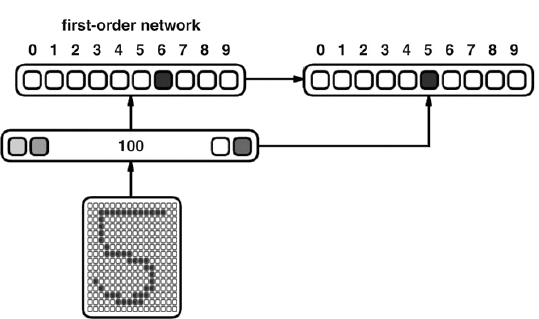
\includegraphics[width=250px]{data/expF5/schema.png}
      \end{center}
      
    \paragraph{Paramètres}
      \begin{center}
	\begin{tabular}{lr}
	  \begin{minipage}{230px}
	    \begin{itemize}
	      \item momentum : 0.5 sur le premier réseau
	      \item momentum : 0. sur le 2\up{ème} réseau
	      \item taux d'apprentissage : 0.15 sur le premier réseau
	      \item taux d'apprentissage : 0.1 sur 2\up{ème} réseau
	      \item \textbf{1600 formes} de chiffres différents présentées (shuffle) \cite{Handwritten_256}
	      
	      
	    \end{itemize}
	  \end{minipage}
	  &
	  \begin{minipage}{230px}
	    \begin{itemize}
	      \item poids initialisés sur [-1 ; 1] pour le premier réseau
	      \item poids initialisés sur [-0.25 ; 0.25] pour le 2\up{ème} réseau
	      \item taux d'apprentissage constant
	      \item entrées valent 0 ou 1
	      \item sigmoïde à température 1
	      \item utilisation de biais
	      \item apprentissage 50 (formes) x 300 (époques)
	    \end{itemize}
	  \end{minipage}
	\end{tabular}
      \end{center}
  
  \newpage
  \subsection{Résultats}
    \paragraph{Principaux}
      Analyse des performances
      \begin{center}
	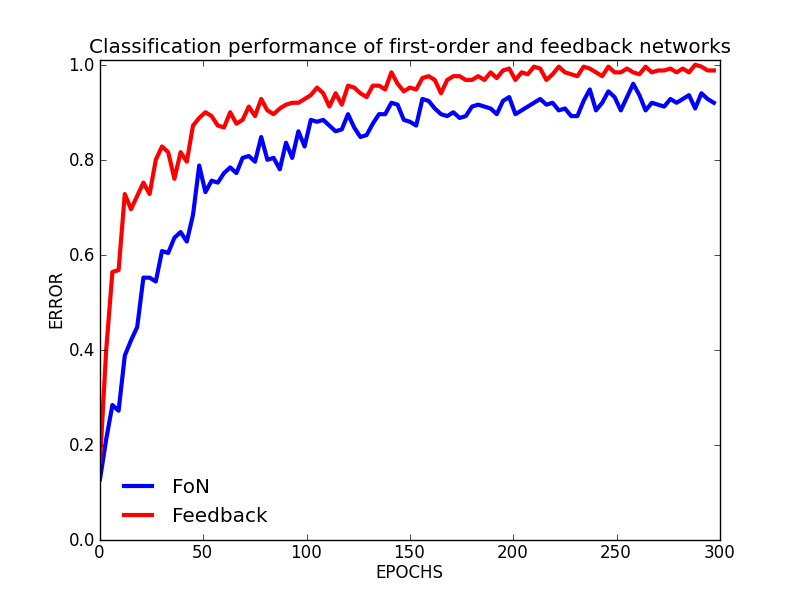
\includegraphics[width=250px]{data/expF5/perff.png}
      \end{center}
      \subparagraph{Notes}
	\begin{itemize}
	  \item La performance de classification représente le taux de bonnes réponses (winner-take-all) pour les 50 formes présentées sur une époque
	\end{itemize}
      \subparagraph{Conclusion}
	\begin{itemize}
	  \item Il y a une très belle hausse de performance toute au long de l'apprentissage
	\end{itemize}


  \subsection{Conclusion}
  Cette belle hausse de performance est très étrange car elle \textbf{remet en cause l'utilité du second réseau et des paris.}
  
  

  \newpage 
  \subsection{Formules}
    \paragraph{Descente de gradient} \cite{Touzet_1992} \\
  Construction de l'erreur : 
    \begin{center}
      $y_{i} = f'(a_i) \times ( d_i - x_i ) \ si\ i\ neurone\ de\ sortie $ \\
      $y_{i} = f'(a_i) \times \sum \limits_{k} ( w_{ki} \times y_k )\ si\ i\ neurone\ cache $
    \end{center}
  Mise à jour des poids :
    \begin{center}
      $w_{ij}(t+1) = w_{ij}(t) + learning\_rate \times y_{i} \times x_j + momentum \times 
      (w_{ij}(t) - w_{ij}(t-1) )$
    \end{center}
  Variables : 
    \begin{center}
      $\left\lbrace \begin{array}{lll} 
	f : fonction\ sigmoide \\
	x_i : valeur\ du\ neurone\ i\\
	d_i : valeur\ desire pour\ le\ neurone\ i\\
	a_i : somme\ pondere\ des\ poids\ du\ neurone\ i
      \end{array} \right.$
    \end{center}
    
\bibliographystyle{../pre-rapport/apalike}
\bibliography{../pre-rapport/biblio}
